
%(BEGIN_QUESTION)
% Copyright 2009, Tony R. Kuphaldt, released under the Creative Commons Attribution License (v 1.0)
% This means you may do almost anything with this work of mine, so long as you give me proper credit

Numerically integrate the following function of $x$ for two different intervals:

$$\includegraphics[width=15.5cm]{i04296x01.eps}$$

\vskip 50pt

$$\int_{4}^{11} f(x) \> dx = $$

\vskip 50pt

$$\int_{18}^{12} f(x) \> dx = $$

\vfil 

\underbar{file i04296}
\eject
%(END_QUESTION)





%(BEGIN_ANSWER)

This is a graded question -- no answers or hints given!

%(END_ANSWER)





%(BEGIN_NOTES)

The general principle to keep in mind here is that integral is the area bounded by a function over some specified interval.  Therefore, in this problem we are looking for the geometrical area underneath the function between $x=4$ and $x=11$ (going forward with positive $dx$ values), as well as between $x=12$ and $x=18$ (going backward with negative $dx$ values):

$$\includegraphics[width=15.5cm]{i04296x02.eps}$$

$$\int_{4}^{11} f(x) \> dx = {\bf 10}$$

\vskip 50pt

$$\int_{18}^{12} f(x) \> dx = {\bf -48.283}$$

%INDEX% Mathematics, calculus: integration (numerical)

%(END_NOTES)


